%%%%%%%%%%%%%%%%%%%%%%%%%%%%%%%%%%%%%%%%%%%%%%
%Includes + Defines
%%%%%%%%%%%%%%%%%%%%%%%%%%%%%%%%%%%%%%%%%%%%%%

%\usepackage{color, colortbl}
%\usepackage{trfsigns}
%\usepackage{graphicx}
%\usepackage{adjustbox}
%\definecolor{TabularBackgroundColor}{rgb}{0.83,0.96,0.96}


%%%%%%%%%%%%%%%%%%%%%%%%%%%%%%%%%%%%%%%%%%%%%%
%Content
%%%%%%%%%%%%%%%%%%%%%%%%%%%%%%%%%%%%%%%%%%%%%%

\section{Wichtige Funktionen}

\small

\subsubsection*{Diracimpuls \tiny (auch Impuls-/Deltafunktion,-Distribution)}

{\footnotesize
Unendlich kurzer, normierter Impuls mit unendlicher Amplitude. }

\begin{multicols}{2}
  \resizebox{0.45\textwidth}{!}{%
    \begin{tabular}{ccl}
      \hline \rowcolor{TabularBackgroundColor}
      1.  & $\delta(-t) = \delta(t) $                                                                                            & gerade Funktion                        \\
      \hline
      2.  & $\delta(-t+t_0) = \delta(t-t_0)$                                                                                     & symmetrisch                            \\
      \hline \rowcolor{TabularBackgroundColor}
      3.  & $\delta(at)= \frac{1}{|a|}\delta(t)$                                                                                 & Skalierung                             \\
      \hline
      4.  & $\delta(\frac{t-t_0}{a}) = |a| \cdot \delta(t-t_0)$                                                                  & Skalierung und Verschiebung            \\
      \hline \rowcolor{TabularBackgroundColor}
      5.  & $\delta(t-t_0)f(t) = f(t_0)\delta(t-t_0)$                                                                            & Abtastung                              \\
      \hline
      6.  & $\int \limits _{-\infty} ^{\infty} \delta(t-t_0)f(t)dt = f(t_0)$                                                     & Siebungseigenschaft                    \\
      \hline \rowcolor{TabularBackgroundColor}
      7.  & $\int \limits _{-\infty} ^{\infty}  A\cdot \delta(t)dt = A$                                                          & Spezialfall Siebungseigenschaft        \\
      \hline
      8.  & $\delta(t-t_0) * f(t) = f(t-t_0)$                                                                                    & Faltung                                \\
      \hline \rowcolor{TabularBackgroundColor}
      9.  & $\delta(t-t_1) * \delta(t-t_2) = \delta(t-t_1-t_2)$                                                                  & Faltung                                \\
    \end{tabular}}
    \resizebox{0.45\textwidth}{!}{%
    \begin{tabular}{ccl}
      \hline
      10. & $\delta(t) = \frac{du(t)}{dt}$                                                                                       & Ableitung Einheitssprung               \\
      \hline \rowcolor{TabularBackgroundColor}
      11. & $ \delta(t) = \lim _{\omega \to \infty} \frac{sin(\omega t)}{\pi t} $                                                & Definition                             \\
      \hline
      12. & $ \delta(t) = \lim _{\epsilon \to \infty} \frac{\epsilon}{\pi(t^2 + \epsilon^2)} $                                   & Definition                             \\
      \hline \rowcolor{TabularBackgroundColor}
      13. & $\delta(t) = \lim _{\epsilon \to 0} \frac{e^{-t^2/\epsilon}}{\sqrt{(\pi \epsilon)}} $                                & Definition                             \\
      \hline
      14. & $t^n \frac{d^n \delta(t)}{dt^n} = (-1)^n n! \delta(t)$                                                               & Ableitung                              \\
      \hline \rowcolor{TabularBackgroundColor}
      15. & $f(t) * \frac{d\delta(t-t_0)}{dt} = \frac{df(t-t_0)}{dt}$                                                            & Faltung mit Ableitung                  \\
      \hline
      16. & $\frac{d\delta(t)}{dt} = \frac{\delta(t)}{-t} = \lim _{\epsilon \to 0} \frac{-2\epsilon t}{\pi(t^2 + \epsilon^2)^2}$ & 1. Ableitung $\delta(t)$ = ungerade F. \\
      \hline \rowcolor{TabularBackgroundColor}
      17. & $1$ \laplace $2\pi\delta(\omega)$                                                                                    & Fourier                                \\
      \hline
      18. & $\delta(t)$ \laplace $1(\omega)$                                                                                         & Fourier                                \\
    \end{tabular}}
\end{multicols}
\resizebox{0.9\textwidth}{!}{%
\begin{tabular}{|p{3.5cm}|p{3.5cm}|p{2cm}|p{3cm}|p{3.5cm}|}
  \hline

  \textbf{Name}
   &
  \textbf{Definition}
   &
  \laplace
   &
  \textbf{Formelzeichen}
   &
  \textbf{plot}
  \\
  \hline
  Sprungfunktion
  \newline (Heaviside)
   &
  $\begin{cases}
       0 \textrm{ für }  t<0,               \\
       [\frac{1}{2} \textrm{ für }  t = 0,] \\
       1 \textrm{ für }  t >0.
     \end{cases}$
  \newline \tiny(machmal: 1 für $t=0$)
   &
  $\frac{1}{j\omega} + \pi\delta(\omega)$
   &
  $u(t), \sigma(t), h(t)$
   &
  \raisebox{-.5\height}{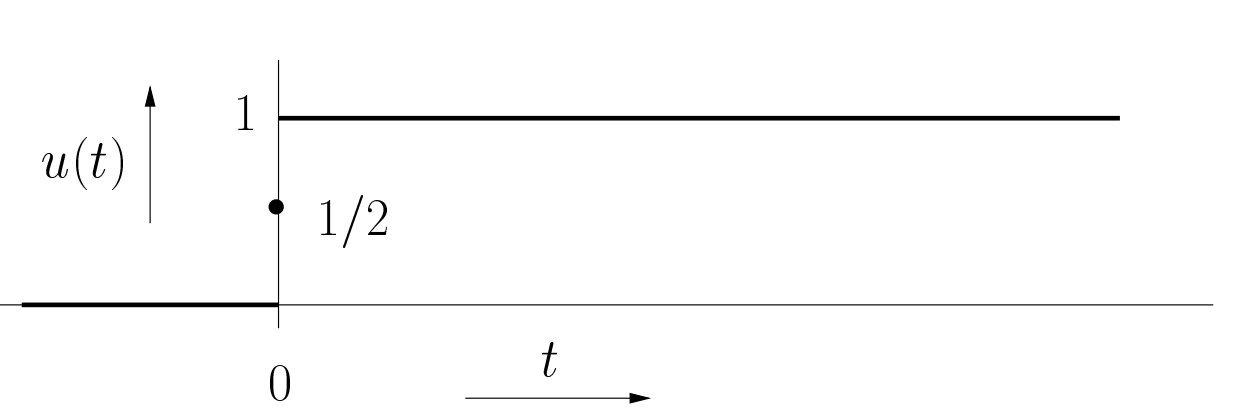
\includegraphics[width = 3.5cm]{include/Wichtige Funktionen/img/Sprungfunktion.png}}
  \\
  Signumfunktion
  \newline (Vorzeichenfunktion)
   &
  $\begin{cases}
       -1 \textrm{ für }  t<0,  \\
       0 \textrm{ für }  t = 0, \\
       1 \textrm{ für }  t >0.
     \end{cases}   $
   &
  $\frac{2}{j\omega}$
   &
  $sgn(t)$
   &
  \raisebox{-.5\height}{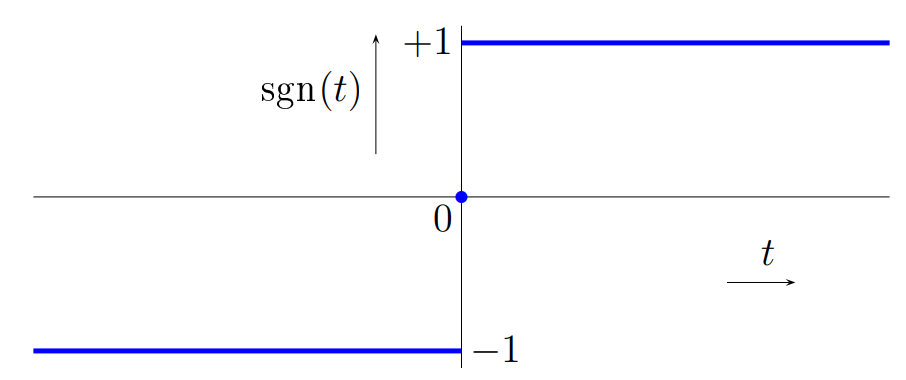
\includegraphics[width=3.5cm]{include/Wichtige Funktionen/img/Signumfunktion.png}}
  \\
  Rampenfunktion
   &
  $\begin{cases}
       0 \textrm{ für } t \leq 0, \\
       t \textrm{ für } t > 0.
     \end{cases}$
   &
  $\frac{1}{s^2}$
   &
  $r(t)$
   &
  \raisebox{-.5\height}{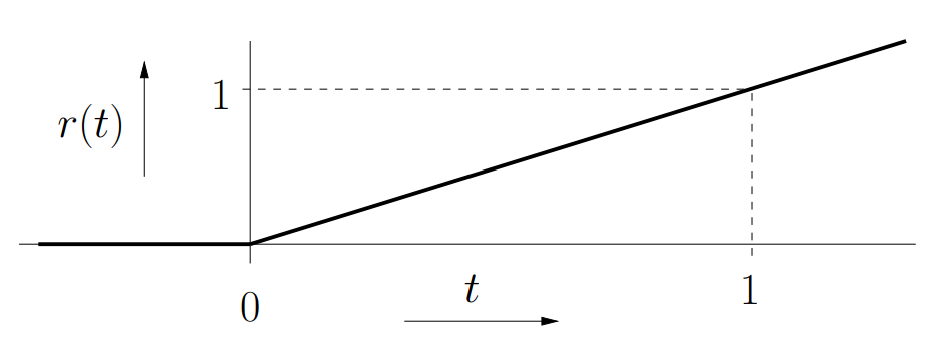
\includegraphics[width=3.5cm]{include/Wichtige Funktionen/img/Rampenfunktion.png}}
  \\
  Rechteckimpuls
   &
  $\begin{cases}
       1 \textrm{ für } |t| < a,           \\
       \frac{1}{2} \textrm{ für } |t| = a, \\
       0 \textrm{ für } |t| > a.
     \end{cases} $
   &
  $\frac{1}{s}- e^{-as}\frac{1}{s} $
   &
  $p_a(t), \beta(t)$
  \newline $\sigma(t+a)-\sigma(t-a)$
   &
  \raisebox{-.5\height}{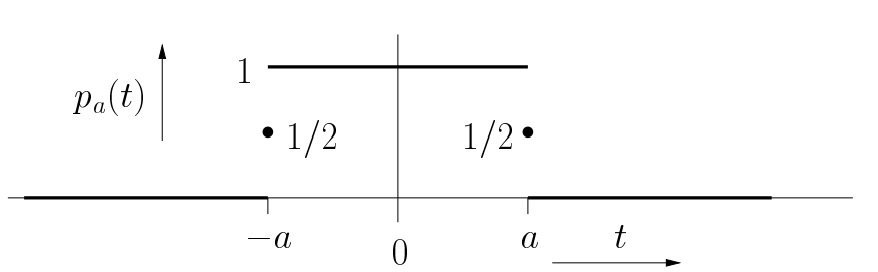
\includegraphics[width=3.5cm]{include/Wichtige Funktionen/img/Rechteckimpuls.png}}
  \\
  Dreieckimpuls
   &
  $\begin{cases}
       1 - \frac{|t|}{a} \textrm{ für } |t| < a \\
       0 \textrm{ für } |t| \geq a
     \end{cases}$
   &
  $sinc^2(\omega)$
   &
  $\Lambda(t)$
   &
  \raisebox{-.5\height}{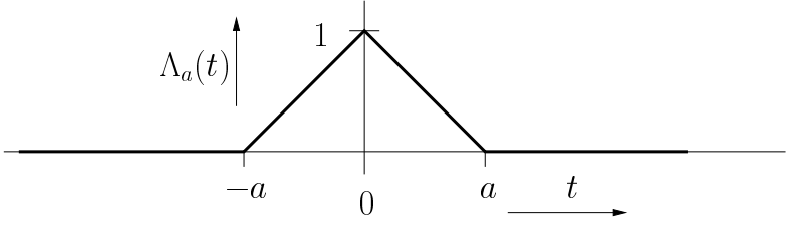
\includegraphics[width=3.5cm]{include/Wichtige Funktionen/img/Dreieckimpuls.png}}
  \\
  Sinc-Funktion
   &
  $\frac{sin(t)}{t}\; \forall t$
  \newline {\tiny $\lim _{t \to 0} sinc(t) = 1$}
  \newline {\tiny wenn normalisiert: $t \to \pi t$}
   &
  $\beta(\omega)$
  \newline{\tiny(Rechteckimpuls)}
   &
  sinc(t)
   &
  \raisebox{-.5\height}{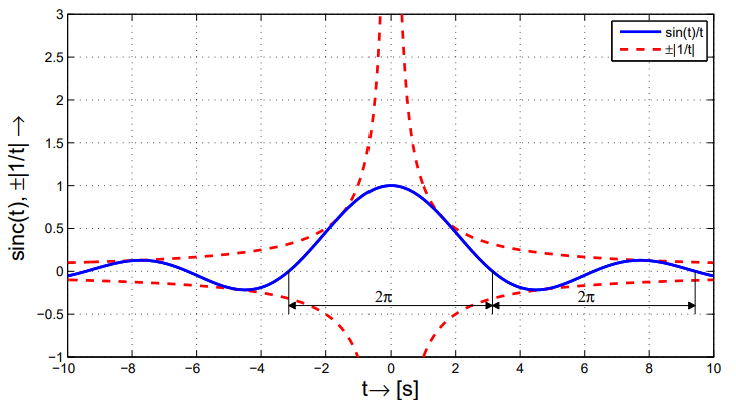
\includegraphics[width=3.5cm]{include/Wichtige Funktionen/img/SincFunktion.png}}
  \\
  \hline
\end{tabular}}